\documentclass[aspectratio=169]{beamer}

\usepackage{xcolor}
\usepackage[T1]{fontenc}
\usepackage{tikz}
\usepackage{array}
\usetikzlibrary{positioning, arrows.meta, shapes.multipart}

% Define custom colors as requested
\definecolor{BgGreen}{HTML}{005D1E}
\definecolor{FooterGreen}{HTML}{88E788}

% Apply colors to beamer elements
\setbeamercolor{background canvas}{bg=BgGreen}
\setbeamercolor{normal text}{fg=white}
\setbeamercolor{structure}{fg=white}
\setbeamercolor{frametitle}{fg=white}
\setbeamercolor{title}{fg=white}
\setbeamercolor{subtitle}{fg=white}
\setbeamercolor{author}{fg=white}
\setbeamercolor{date}{fg=white}
\setbeamercolor{itemize item}{fg=FooterGreen}
\setbeamercolor{itemize subitem}{fg=FooterGreen}

% Configure central footer
\setbeamertemplate{footline}{
    \leavevmode%
    \hbox{%
        \begin{beamercolorbox}[wd=\paperwidth,ht=3ex,dp=1.5ex,center]{}%
            \color{FooterGreen}\tiny Sustainable Software Engineering - 2Chance Web Application
        \end{beamercolorbox}%
    }%
    \vskip0pt%
}

% Remove default navigation symbols
\setbeamertemplate{navigation symbols}{}

% Font configuration 
% Using Comfortaa, a rounded sans-serif font similar to Fredoka that works with pdflatex
\usepackage[default]{comfortaa}

\begin{document}

\begin{frame}
    \begin{center}
        \vspace*{0.5cm}
        \textcolor{FooterGreen}{\LARGE \textbf{Green Refactoring of the \\
        2chance Web Application: \\
        An Empirical Analysis of \\
        Energy Patterns and Performance}}
        
        \vspace{1.5cm}
        
        \textcolor{FooterGreen}{\small Sustainable Software Engineering \\
        Green-in-Software Project}
    \end{center}
\end{frame}
\begin{frame}
    \begin{center}
        \textcolor{FooterGreen}{\LARGE \textbf{2Chance Web Application}}
        \vspace{0.8cm}
        
        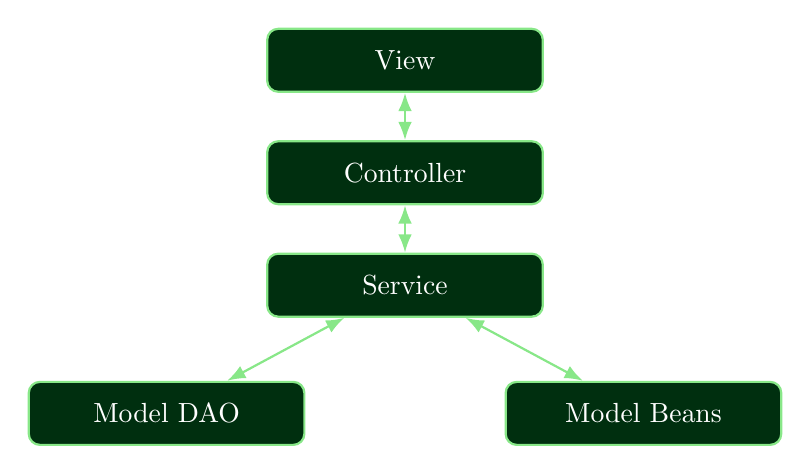
\begin{tikzpicture}[
            node distance=0.6cm and 1cm,
            box/.style={draw=FooterGreen, thick, rounded corners, text=white, minimum width=3.5cm, minimum height=0.8cm, align=center, fill=BgGreen!50!black},
            arrow/.style={<->, thick, FooterGreen, >=Latex}
        ]
            
            \node[box] (view) {View};
            \node[box, below=of view] (controller) {Controller};
            \node[box, below=of controller] (service) {Service};
            
            \node[box, below left=0.8cm and -0.5cm of service] (dao) {Model DAO};
            \node[box, below right=0.8cm and -0.5cm of service] (beans) {Model Beans};
            
            \draw[arrow] (view) -- (controller);
            \draw[arrow] (controller) -- (service);
            \draw[arrow] (service) -- (dao);
            \draw[arrow] (service) -- (beans);
            
        \end{tikzpicture}
    \end{center}
\end{frame}

\begin{frame}
    \begin{center}
        \textcolor{FooterGreen}{\LARGE \textbf{View}}
        \vspace{0.8cm}
        
        
\begin{tikzpicture}[
            node distance=0.8cm and 1cm,
            box/.style={draw=FooterGreen, thick, rounded corners, text=white, minimum width=4.5cm, minimum height=1cm, align=center, fill=BgGreen!50!black},
            desc/.style={text=white, text width=8cm, align=left, font=\small}
        ]
            
            \node[box] (ui) {HTML, CSS};
            \node[desc, right=of ui] {INTERFACCIA UTENTE (UI)};
            
            \node[box, below=of ui] (interactive) {JavaScript};
            \node[desc, right=of interactive] {INTERATTIVITÀ LATO CLIENT E \\ ACQUISIZIONE DEGLI INPUT DELL'UTENTE};
            
            \node[box, below=of interactive] (dynamic) {JavaServer Pages (JSP)};
            \node[desc, right=of dynamic] {VISUALIZZARE DINAMICAMENTE DATI \\ FORNITI DAL CONTROLLER};
            
        \end{tikzpicture}
    \end{center}
\end{frame}

\begin{frame}
    \begin{center}
        \textcolor{FooterGreen}{\LARGE \textbf{Controller + Service}}
        \vspace{0.8cm}
        
        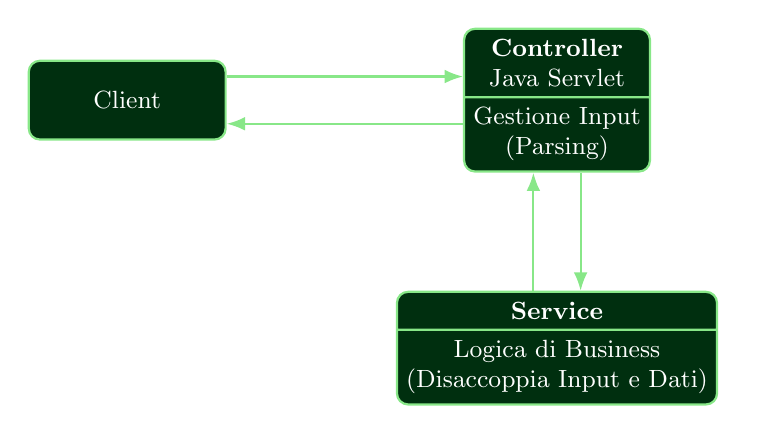
\begin{tikzpicture}[
            node distance=3cm,
            box/.style={draw=FooterGreen, thick, rounded corners, text=white, minimum width=2.5cm, minimum height=1cm, align=center, fill=BgGreen!50!black, font=\small},
            splitbox/.style={draw=FooterGreen, thick, rounded corners, text=white, align=center, fill=BgGreen!50!black, rectangle split, rectangle split parts=2, rectangle split part fill={BgGreen!50!black, BgGreen!70!black}, font=\small},
            arrow/.style={->, thick, FooterGreen, >=Latex},
            lbl/.style={text=white, font=\tiny, align=center}
        ]
            
            \node[box] (client) {Client};
            
            \node[splitbox, right=of client] (controller) {
                \textbf{Controller} \\ Java Servlet
                \nodepart{two}
                Gestione Input \\ (Parsing)
            };
            
            \node[splitbox, below=1.5cm of controller] (service) {
                \textbf{Service}
                \nodepart{two}
                Logica di Business \\ (Disaccoppia Input e Dati)
            };
            
            \draw[arrow] ([yshift=3mm]client.east) -- ([yshift=3mm]controller.west) node[midway, above, lbl] {Richiesta \\ HTTP};
            \draw[arrow] ([yshift=-3mm]controller.west) -- ([yshift=-3mm]client.east) node[midway, below, lbl] {Forward a JSP \\ (Rendering)};
            
            \draw[arrow] ([xshift=3mm]controller.south) -- ([xshift=3mm]service.north) node[midway, right, lbl] {Delega \\ (Invoca Metodi)};
            \draw[arrow] ([xshift=-3mm]service.north) -- ([xshift=-3mm]controller.south) node[midway, left, lbl] {Risultato \\ Elaborazione};
            
        \end{tikzpicture}
    \end{center}
\end{frame}

\begin{frame}
    \begin{center}
        \textcolor{FooterGreen}{\LARGE \textbf{Model Data Access Object (DAO)}}
        
        \vspace{0.4cm}
        \textcolor{white}{\textit{``Astrae e incapsula tutto l'accesso al database che contiene i dati persistenti.''}}
        \vspace{0.8cm}
        
        
\begin{tikzpicture}[
            splitbox/.style={draw=FooterGreen, thick, rounded corners, text=white, align=center, fill=BgGreen!50!black, rectangle split, rectangle split parts=2, rectangle split part fill={BgGreen!50!black, BgGreen!70!black}, font=\small},
            desc/.style={text=white, text width=8cm, align=left, font=\small},
            arrow/.style={->, thick, FooterGreen, >=Latex}
        ]
            
            \node[splitbox] (db) {JDBC \nodepart{two} Tomcat Connection Pool};
            
            \node[desc, above right=0.8cm and 1cm of db.east, anchor=west] (crud) {
                \textbf{Operazioni CRUD:} \\ Esecuzione di transazioni Create, Read, Update e Delete.
            };
            
            \node[desc, below right=0.8cm and 1cm of db.east, anchor=west] (orm) {
                \textbf{Object--Relational Mapping (ORM):} \\ Trasformazione di dati relazionali grezzi (es. \texttt{ResultSet}) in oggetti Java ad alto livello (Model Bean) e viceversa.
            };
            
            \draw[arrow] (db.east) -- (crud.west);
            \draw[arrow] (db.east) -- (orm.west);
            
        \end{tikzpicture}
    \end{center}
\end{frame}

\begin{frame}
    \begin{center}
        \textcolor{FooterGreen}{\LARGE \textbf{Software Dependability Improvements}}
        \vspace{0.8cm}
        
        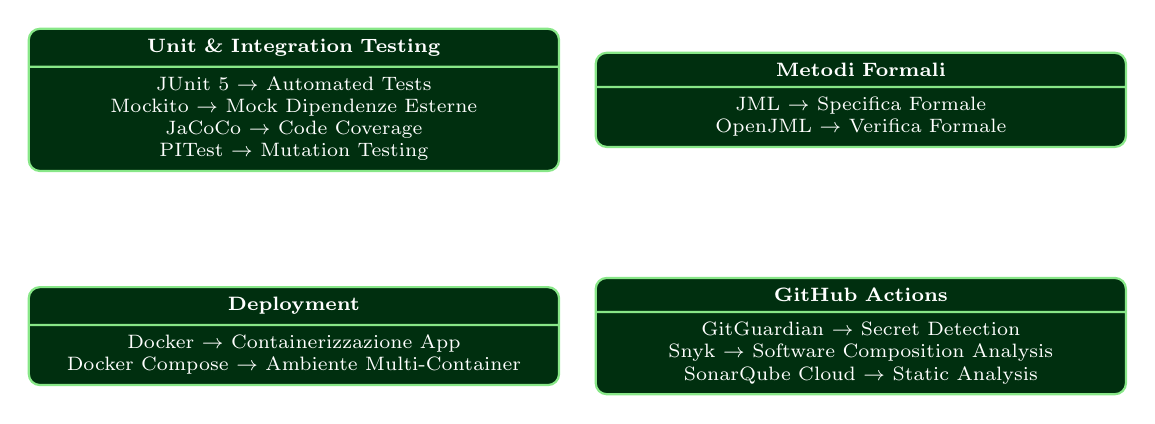
\begin{tikzpicture}[
            splitbox/.style={draw=FooterGreen, thick, rounded corners, text=white, align=center, fill=BgGreen!50!black, rectangle split, rectangle split parts=2, rectangle split part fill={BgGreen!50!black, BgGreen!70!black}, font=\scriptsize, text width=6.5cm, minimum height=2.5cm}
        ]
            
            \node[splitbox] at (-3.6, 0) (testing) {
                \textbf{Unit \& Integration Testing}
                \nodepart{two}
                JUnit 5 $\rightarrow$ Automated Tests \\
                Mockito $\rightarrow$ Mock Dipendenze Esterne \\
                JaCoCo $\rightarrow$ Code Coverage \\
                PITest $\rightarrow$ Mutation Testing
            };
            
            \node[splitbox] at (3.6, 0) (formal) {
                \textbf{Metodi Formali}
                \nodepart{two}
                JML $\rightarrow$ Specifica Formale \\
                OpenJML $\rightarrow$ Verifica Formale
            };
            
            \node[splitbox] at (-3.6, -3) (deploy) {
                \textbf{Deployment}
                \nodepart{two}
                Docker $\rightarrow$ Containerizzazione App \\
                Docker Compose $\rightarrow$ Ambiente Multi-Container
            };
            
            \node[splitbox] at (3.6, -3) (actions) {
                \textbf{GitHub Actions}
                \nodepart{two}
                GitGuardian $\rightarrow$ Secret Detection \\
                Snyk $\rightarrow$ Software Composition Analysis \\
                SonarQube Cloud $\rightarrow$ Static Analysis
            };
            
        \end{tikzpicture}
    \end{center}
\end{frame}

\begin{frame}
    \begin{center}
        \textcolor{FooterGreen}{\LARGE \textbf{Backend Energy Sustainability}}
        \vspace{0.8cm}
        
        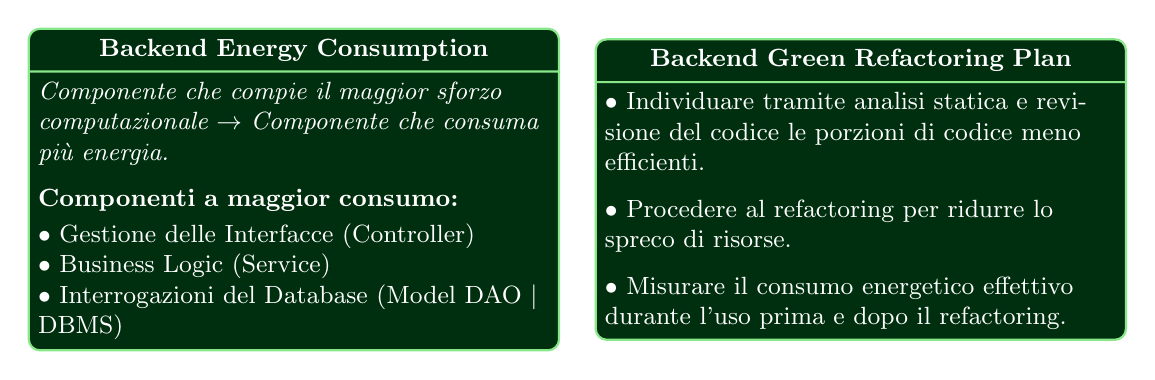
\begin{tikzpicture}[
            splitbox/.style={draw=FooterGreen, thick, rounded corners, text=white, align=left, fill=BgGreen!50!black, rectangle split, rectangle split parts=2, rectangle split part fill={BgGreen!50!black, BgGreen!70!black}, font=\small, text width=6.5cm}
        ]
            
            \node[splitbox] at (-3.6, 0) (leftbox) {
                \centering \textbf{Backend Energy Consumption} \\
                \nodepart{two}
                \textit{Componente che compie il maggior sforzo computazionale $\rightarrow$ Componente che consuma più energia.}\\[1.5ex]
                \textbf{Componenti a maggior consumo:}\\[0.5ex]
                $\bullet$ Gestione delle Interfacce (Controller) \\
                $\bullet$ Business Logic (Service) \\
                $\bullet$ Interrogazioni del Database (Model DAO $|$ DBMS)
            };
            
            \node[splitbox] at (3.6, 0) (rightbox) {
                \centering \textbf{Backend Green Refactoring Plan} \\
                \nodepart{two}
                $\bullet$ Individuare tramite analisi statica e revisione del codice le porzioni di codice meno efficienti.\\[1.5ex]
                $\bullet$ Procedere al refactoring per ridurre lo spreco di risorse.\\[1.5ex]
                $\bullet$ Misurare il consumo energetico effettivo durante l'uso prima e dopo il refactoring.
            };
            
        \end{tikzpicture}
    \end{center}
\end{frame}

\begin{frame}
    \begin{center}
        \textcolor{FooterGreen}{\LARGE \textbf{Rule-Based Eco-Design Static Analysis}}
        \vspace{0.8cm}
        
        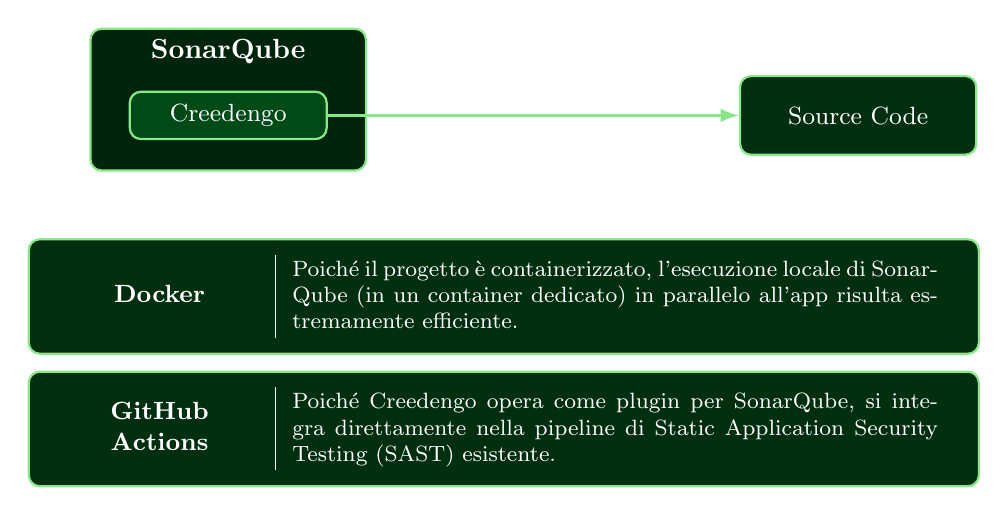
\begin{tikzpicture}[
            box/.style={draw=FooterGreen, thick, rounded corners, text=white, align=center, fill=BgGreen!50!black, font=\small, minimum height=1cm},
            desc/.style={text=white, text width=7.5cm, align=left, font=\small},
            arrow/.style={->, thick, FooterGreen, >=Latex}
        ]
            
            % Top part: SonarQube -> Creedengo -> Source Code
            \node[draw=FooterGreen, thick, rounded corners, text=white, align=center, fill=BgGreen!40!black, minimum width=3.5cm, minimum height=1.8cm] at (-3, 0) (sonar) {};
            \node[text=white, font=\bfseries] at ([yshift=-0.3cm]sonar.north) {SonarQube};
            \node[box, fill=BgGreen!80!black, minimum width=2.5cm, minimum height=0.6cm] (creedengo) at ([yshift=-0.2cm]sonar.center) {Creedengo};
            
            \node[box, minimum width=3cm] at (5, -0.2) (code) {Source Code};
            
            \draw[arrow] (creedengo) -- (code) node[midway, above, text=white, font=\tiny, align=center] {Ricerca di Anti-Pattern Energetici};
            
            % Middle part: Docker
            \node[box, inner sep=0.2cm] at (0.5, -2.5) (docker) {
                \begin{tabular}{>{\centering\arraybackslash}m{2.5cm} | m{8.2cm}}
                    \textbf{Docker} & \footnotesize Poiché il progetto è containerizzato, l'esecuzione locale di SonarQube (in un container dedicato) in parallelo all'app risulta estremamente efficiente.
                \end{tabular}
            };
            
            % Bottom part: GitHub Actions
            \node[box, inner sep=0.2cm, below=0.2cm of docker] (gh) {
                \begin{tabular}{>{\centering\arraybackslash}m{2.5cm} | m{8.2cm}}
                    \textbf{GitHub Actions} & \footnotesize Poiché Creedengo opera come plugin per SonarQube, si integra direttamente nella pipeline di Static Application Security Testing (SAST) esistente.
                \end{tabular}
            };
            
        \end{tikzpicture}
    \end{center}
\end{frame}

\begin{frame}
    \begin{center}
        \textcolor{FooterGreen}{\Large \textbf{Configurazione con Script Automatico di SonarQube con il Plugin Creedengo}}
        \vspace{0.2cm}
        
        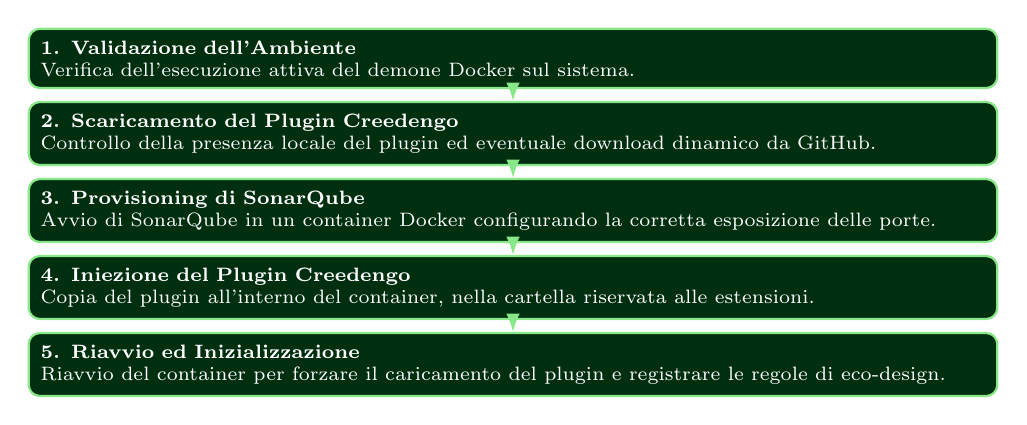
\begin{tikzpicture}[
            stepbox/.style={draw=FooterGreen, thick, rounded corners, text=white, fill=BgGreen!50!black, align=left, text width=12cm, font=\scriptsize, inner sep=0.15cm},
            arrow/.style={->, thick, FooterGreen, >=Latex}
        ]
            \node[stepbox] (step1) {\textbf{1. Validazione dell'Ambiente} \\ Verifica dell'esecuzione attiva del demone Docker sul sistema.};
            \node[stepbox, below=0.15cm of step1] (step2) {\textbf{2. Scaricamento del Plugin Creedengo} \\ Controllo della presenza locale del plugin ed eventuale download dinamico da GitHub.};
            \node[stepbox, below=0.15cm of step2] (step3) {\textbf{3. Provisioning di SonarQube} \\ Avvio di SonarQube in un container Docker configurando la corretta esposizione delle porte.};
            \node[stepbox, below=0.15cm of step3] (step4) {\textbf{4. Iniezione del Plugin Creedengo} \\ Copia del plugin all'interno del container, nella cartella riservata alle estensioni.};
            \node[stepbox, below=0.15cm of step4] (step5) {\textbf{5. Riavvio ed Inizializzazione} \\ Riavvio del container per forzare il caricamento del plugin e registrare le regole di eco-design.};
            
            \draw[arrow] (step1) -- (step2);
            \draw[arrow] (step2) -- (step3);
            \draw[arrow] (step3) -- (step4);
            \draw[arrow] (step4) -- (step5);
            
        \end{tikzpicture}
    \end{center}
\end{frame}

\begin{frame}
    \begin{center}
        \textcolor{FooterGreen}{\LARGE \textbf{Selezione delle Regole di Eco-Design}}
        \vspace{0.4cm}
        
        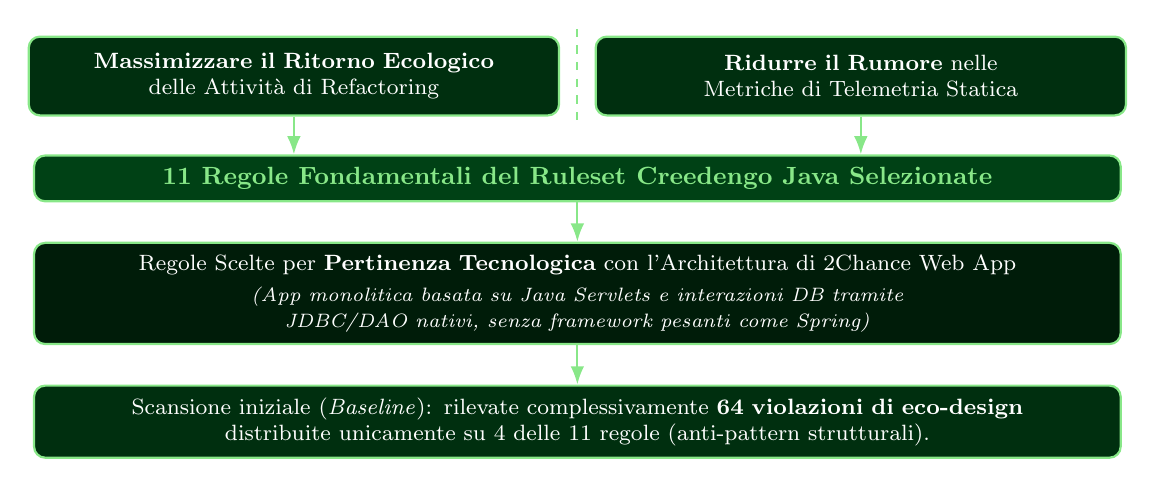
\begin{tikzpicture}[
            box/.style={draw=FooterGreen, thick, rounded corners, text=white, align=center, fill=BgGreen!50!black, font=\footnotesize, text width=6.5cm, minimum height=1cm},
            arrow/.style={->, thick, FooterGreen, >=Latex},
            desc/.style={draw=FooterGreen, thick, rounded corners, text=white, align=center, fill=BgGreen!50!black, font=\footnotesize, text width=13.5cm, inner sep=0.15cm}
        ]
            
            % Top part
            \node[box] at (-3.6, 0) (leftbox) {\textbf{Massimizzare il Ritorno Ecologico} \\ delle Attività di Refactoring};
            
            \draw[thick, FooterGreen, dashed] (0, 0.6) -- (0, -0.6);
            
            \node[box] at (3.6, 0) (rightbox) {\textbf{Ridurre il Rumore} nelle \\ Metriche di Telemetria Statica};
            
            % Middle part 1
            \node[desc, font=\bfseries\small, text=FooterGreen, fill=BgGreen!70!black] at (0, -1.3) (regole) {11 Regole Fondamentali del Ruleset Creedengo Java Selezionate};
            
            % Arrows from top to middle
            \draw[arrow] (leftbox.south) -- (leftbox.south |- regole.north);
            \draw[arrow] (rightbox.south) -- (rightbox.south |- regole.north);
            
            % Middle part 2 (formerly bottom part)
            \node[desc, fill=BgGreen!30!black, below=0.5cm of regole] (arch) {Regole Scelte per \textbf{Pertinenza Tecnologica} con l'Architettura di 2Chance Web App \\[0.5ex] \scriptsize \textit{(App monolitica basata su Java Servlets e interazioni DB tramite JDBC/DAO nativi, senza framework pesanti come Spring)}};
            
            \draw[arrow] (regole.south) -- (arch.north);
            
            % Bottom part (new baseline node)
            \node[desc, fill=BgGreen!50!black, below=0.5cm of arch] (baseline) {Scansione iniziale (\textit{Baseline}): rilevate complessivamente \textbf{64 violazioni di eco-design} \\ distribuite unicamente su 4 delle 11 regole (anti-pattern strutturali).};
            
            \draw[arrow] (arch.south) -- (baseline.north);
            
        \end{tikzpicture}
    \end{center}
\end{frame}

\end{document}
